\documentclass{beamer}

\newenvironment{tightcenter}{%
  \setlength\topsep{0pt}
  \setlength\parskip{0pt}
  \begin{center}
}{%
  \end{center}
}

\mode<presentation>
{
  \usetheme{Copenhagen}
  %%\usecolortheme[RGB={173,222,25}]{structure}
  \usecolortheme[RGB={255,0,0}]{structure}
  \setbeamertemplate{items}[circle]
  \setbeamercovered{transparent}
}

\usepackage[polish]{babel}
\usepackage{chessfss}
\usepackage{hyperref}
\usepackage{qtree}
\usepackage{mathtools}
\usepackage{dirtytalk}
\usepackage{epigraph}
\usepackage{textgreek}
\usepackage[utf8]{inputenc}
\usepackage{times}
\usepackage[T1]{fontenc}
\usepackage{tikz}
\usepackage{csquotes}
\usepackage{amsmath}
\usepackage{fancyvrb}
\usepackage{ulem}
\usepackage{adjustbox}

\newenvironment{Snippet}{\Verbatim[samepage=true]}{\endVerbatim}

\title{\textbf{The Ultimatest Monad Tutorial}}

\author{Panicz Maciej Godek}

\institute{
  \tiny{\href{mailto:godek.maciek@gmail.com}{\textbf{godek.maciek@gmail.com}}}
}

\date{15.12.2023}

\begin{document}

\begin{frame}
  \titlepage
\end{frame}

\begin{frame}{Agenda}
  \begin{itemize}
    \pause \item the concept of monads
    \pause \item problems with Haskell
    \pause \item pyramid of doom (with sugar coating)
    \pause \item rants
  \end{itemize}
\end{frame}

\begin{frame}{Point-free programming}
  Inverse of a square root \\ \pause
  \texttt{isqrt x = 1/(sqrt x)} \\ \pause
  point-free style: \\ \pause
  \texttt{isqrt = (1/) .\ sqrt} \\ \pause
  where
  \texttt{(f .\ g) x = f (g x)} \\ \pause
  in JS: \\
  \texttt{function compose(f, g) \{ \\
    \ \ return function(x) \{ \\
    \ \ \ \ return f(g(x)); \\
    \ \ \}; \\
    \}}  
\end{frame}

\begin{frame}{Function composition operator}
  Type of the function composition operator: \\ \pause
  \texttt{(.) :: (b -> c) -> (a -> b) -> (a -> c)} \\ \pause
  looks a bit awkward, but if we define \\
  \texttt{(g | f) x = f (g x)} \\ \pause
  the type of the ``swapped composition'' is \\ \pause
  \texttt{(|) :: (a -> b) -> (b -> c) -> (a -> c)} \\ \pause
  vide UNIX pipes \\ \pause
  or ``the uncle of the friend of my brother'' vs.\ ``my brother\textquotesingle s friend\textquotesingle s uncle'' \\ \pause
  or \texttt{f(g(x))} vs.\ \texttt{x->getG()->getF()}
\end{frame}

\begin{frame}{Function composition operator}
  Properties of function composition: \pause
  \begin{itemize}
  \item associative: \texttt{f .\ (g .\ h) = (f .\ g) .\ h} \\ \pause
    like: \texttt{x + (y + z) = (x + y) + z} \\ \pause
    or: \texttt{x * (y * z) = (x * y) * z} \pause
  \item has a neutral element \texttt{id}: \\ \pause
    \texttt{f .\ id = id .\ f = f} \\ \pause
    like: \texttt{x + 0 = 0 + x = x} \\ \pause
    or: \texttt{x * 1 = 1 * x = x} \pause
  \end{itemize}
  where the \texttt{id} function is defined as\\
  \texttt{id x = x} \\ \pause
  \texttt{function id(x) \{ return x; \}}
\end{frame}


\begin{frame}{All that math}
  In mathematics, an associative operator with neutral element is called \textit{a monoid}
  (or \textit{semigroup with identity}). \\ \pause
  Now imagine the following \textit{generalization} of the composition operator: \\ \pause
  \texttt{<|$_m$ ::\ (b -> $m$ c) -> (a -> $m$ b) -> (a -> $m$ c)} \\ \pause
  For example: \\
  \texttt{class WithLog<T> \{ \\
    \ \ public T value; \\
    \ \ public String log; \\
    \}} \\ \pause
  \texttt{(f <|$_\mathtt{WithLog}$ g) a = \\
    \ \ WithLog b = g(a); \\
    \ \ WithLog c = f(b.value); \\
    \ \ return WithLog(value = c.value, log = b.log + c.log); }
\end{frame}

\begin{frame}{Generalization of idenity}
  \texttt{id$_\mathtt{WithLog}$ x = WithLog(value = x, log = '''')} \\ \pause
  The triple \texttt{($m$, <|$_m$, id$_m$)} is called \textit{a monad}. \\ \pause
  For example, \texttt{(WithLog, <|$_\mathtt{WithLog}$, id$_\mathtt{WithLog}$)}
  is a monad. \\ \pause
  Other popular examples: \texttt{Optional}, \texttt{List}.

   %% \texttt{(f <|$_\mathtt{List}$ g) a = \\
   %%  \ \ List b = f(a); \\
   %%  \ \ List result = new LinkedList(); \\
   %%  \ \ for (Object x : b) \{ \\
   %%  \ \ \ \ result.addAll(g(x)); \\
   %%  \ \ \} \\
   %%  \ \ return result;}

\end{frame}

\begin{frame}{But why?}
  \pause
  Problem with Haskella: lazy evaluation. \\ \pause
  Solution: ``input/output system based on monads'' \\ \pause
  But what does it mean?
\end{frame}

\begin{frame}{Evaluation strategies}
  \texttt{square x = x * x} \\ \pause
  \ \\
  The ``applicative'' order (evaluate arguments before expanding function): \\ \pause
  \texttt{square (2*3) \pause = square 6 \pause =$_{def}$ 6 * 6 \pause = 36} \\ \pause
  \ \\
  The ``normal'' order (evaluate arguments as late as possible): \\ \pause
  \texttt{square (2*3) \pause =$_{def}$ (2*3) * (2*3) \pause = 6 * 6 \pause = 36}
\end{frame}


\begin{frame}{The problem with Haskell: lazy evaluation}
  \texttt{readNumber()*3 + 2*readNumber()} \\ \pause
  \texttt{\phantom{}< 1} \\ \pause
  \texttt{\phantom{}< 0} \\  
\end{frame}

\begin{frame}{Idea for a solution}
  \texttt{ \\ \ \\
    let \ a\ \ \ \ \  = readNumber(\ \ ) in \\ \pause
    \ \ let \ b\ \ \ \ \ = readNumber(\ \ ) in \\ \pause
    \ \ \ \ \ a*2 + 3*b
  } \\ \pause gdzie \\
  \texttt{\textbf{let} name = value \textbf{in} expression} \\ 
  \texttt{(λ name -> expression) value}
\end{frame}


\begin{frame}{A working solution}
  \texttt{ \\ \ \\
    let (a,w1) = readNumber(w0) in \\
    \ \ let (b,w2) = readNumber(w1) in \\
    \ \ \ \ \ a*2 + 3*b
  } \\ \ \\ \ \\ \ 
\end{frame}

\begin{frame}{A better solution}
  \texttt{ \\ \ \\
    let (a,w1) = readNumber(w0) in \\
    \ \ let (b,w2) = readNumber(w1) in \\
    \ \ \ \ (a*2 + 3*b, w2)
  } \\ \ \\ \ \\ \ 
\end{frame}

\begin{frame}{Extracting a function}
  \texttt{myOperation ::\ RealWorld -> (Int, RealWorld)
    myOperation w0 = \\
    let (a,w1) = readNumber(w0) in \\
    \ \ let (b,w2) = readNumber(w1) in \\
    \ \ \ \ (a*2 + 3*b, w2)
  } \\ \ \\ \ \\ \url{https://wiki.haskell.org/IO_inside}
\end{frame}

\begin{frame}{Problems}
  \pause
  \begin{itemize}
  \item we need to pass additional argument \pause
  \item error-prone (e.g. \texttt{w0} instead of \texttt{w1}) \pause
  \item indentation level increases
  \end{itemize}
\end{frame}

\begin{frame}{Sweeping \texttt{w$_n$} under the rug}
  \texttt{pass readNumber \\
    \ \ \ \ \ (λ a \pause -> pass readNumber \\
    \ \ \ \ \ \ \ \ \ \ \ \ \ \ \ \ \ \ (λ b \pause -> return a*2 + 3*b)) \\
    \ \\ \pause
    return value = λ world -> (value, world) \\ \pause
    \ \\
    pass value continuation = λ w0 -> \\
    \ \ let (result, w1) = value w0 in \\
    \ \ \ \ \ continuation result w1
  }
\end{frame}


\begin{frame}{But does it work?}
  \texttt{pass readNumber\\
    \ \ \ \ \ (λ a -> pass readNumber\\
    \ \ \ \ \ \ \ \ \ \ \ \ \ \ \ \ \ \ (λ b -> \textbf{return a*2 + 3*b}))\\
    \ \\
    \textbf{return value = λ world -> (value, world)} \\
    \ \\
    pass value continuation = λ w0 -> \\
    \ \ let (result, w1) = value w0 in \\
    \ \ \ \ \ continuation result w1
  }
\end{frame}

\begin{frame}{But does it work?}
  \texttt{pass readNumber\\
    \ \ \ \ \ (λ a -> pass readNumber\\
    \ \ \ \ \ \ \ \ \ \ \ \ \ \ (λ b -> \textbf{λ w -> (a*2 + 3*b, w)}))\\
    \ \\
    \textbf{return value = λ world -> (value, world)} \\
    \ \\
    pass value continuation = λ w0 -> \\
    \ \ let (result, w1) = value w0 in \\
    \ \ \ \ \ continuation result w1
  }
\end{frame}

\begin{frame}{But does it work?}
  \texttt{pass readNumber\\
    \ \ \ \ \ (λ a -> \textbf{pass readNumber\\
      \ \ \ \ \ \ \ \ \ \ \ \ \ \ (λ b -> λ w -> (a*2 + 3*b, w))})\\
    \ \\
    return value = λ world -> (value, world) \\
    \ \\
    \textbf{pass value continuation = λ w0 -> \\
      \ \ let (result, w1) = value w0 in \\
      \ \ \ \ \ continuation result w1}
  }
\end{frame}

\begin{frame}{But does it work?}
  \texttt{pass readNumber (λ a -> \textbf{λ w1 -> \\
      \ \ let (y, w2) = readNumber(w1) in\\
      \ \ \ \ \ \ \ \ (λ b -> λ w -> (a*2 + 3*b, w)) y w2})\\
    \ \\
    return value = λ world -> (value, world) \\
    \ \\
    \textbf{pass value continuation = λ w0 -> \\
      \ \ let (result, w1) = value w0 in \\
      \ \ \ \ \ continuation result w1}
  }
\end{frame}

\begin{frame}{But does it work?}
  \texttt{pass readNumber (λ a -> λ w1 -> \\
    \ \ let (y, w2) = readNumber(w1) in\\
    \ \ \ \ \ \ \ \ \ \textbf{(λ b -> λ w -> (a*2 + 3*b, w)) y w2})\\
    \ \\
    return value = λ world -> (value, world) \\
    \ \\
    pass value continuation = λ w0 -> \\
    \ \ let (result, w1) = value w0 in \\
    \ \ \ \ \ continuation result w1
  }
\end{frame}

\begin{frame}{But does it work?}
  \texttt{pass readNumber (λ a -> λ w1 -> \\
    \ \ let (y, w2) = readNumber(w1) in\\
    \ \ \ \ \ \ \ \ \ \textbf{(λ w -> (a*2 + 3*y, w)) w2})\\
    \ \\
    return value = λ world -> (value, world) \\
    \ \\
    pass value continuation = λ w0 -> \\
    \ \ let (result, w1) = value w0 in \\
    \ \ \ \ \ continuation result w1
  }
\end{frame}

\begin{frame}{But does it work?}
  \texttt{pass readNumber (λ a -> λ w1 -> \\
    \ \ let (y, w2) = readNumber(w1) in\\
    \ \ \ \ \ \ \ \ \ \textbf{(a*2 + 3*y, w2)})\\
    \ \\
    return value = λ world -> (value, world) \\
    \ \\
    pass value continuation = λ w0 -> \\
    \ \ let (result, w1) = value w0 in \\
    \ \ \ \ \ continuation result w1
  }
\end{frame}

\begin{frame}{But does it work?}
  \texttt{\textbf{pass readNumber (λ a -> λ w1 ->\\
      \ \ let (y, w2) = readNumber(w1) in\\
      \ \ \ \ \ \ \ \ (a*2 + 3*y, w2))}\\
    \ \\
    return value = λ world -> (value, world) \\
    \ \\
    \textbf{pass value continuation = λ w0 -> \\
      \ \ let (result, w1) = value w0 in \\
      \ \ \ \ \ continuation result w1}
  }
\end{frame}

\begin{frame}{But does it work?}
  \texttt{\textbf{λ w0 -> let (x,w3) = readNumber(w0) in\\
      \ \ (λ a -> λ w1 -> let (y, w2) = readNumber(w1) \\
      \ \ \ \ \ \ in (a*2 + 3*y, w2)) x w3}\\
    \ \\
    return value = λ world -> (value, world) \\
    \ \\
    \textbf{pass value continuation = λ w0 -> \\
      \ \ let (result, w1) = value w0 in \\
      \ \ \ \ \ continuation result w1}
  }
\end{frame}

\begin{frame}{But does it work?}
  \texttt{λ w0 -> let (x,w3) = readNumber(w0) in\\
    \ \ \textbf{(λ a -> λ w1 -> let (y, w2) = readNumber(w1)\\
      \ \ \ \ \ \ in (a*2 + 3*y, w2)) x w3}\\
    \ \\
    return value = λ world -> (value, world) \\
    \ \\
    pass value continuation = λ w0 -> \\
    \ \ let (result, w1) = value w0 in \\
    \ \ \ \ \ continuation result w1
  }
\end{frame}

\begin{frame}{But does it work?}
  \texttt{λ w0 -> let (x,w3) = readNumber(w0) in\\
    \ \ \textbf{(λ w1 -> let (y, w2) = readNumber(w1) in\\
      \ \ \ \ \ \ \ \ \ (x*2 + 3*y, w2)) w3}\\
    \ \\
    return value = λ world -> (value, world) \\
    \ \\
    pass value continuation = λ w0 -> \\
    \ \ let (result, w1) = value w0 in \\
    \ \ \ \ \ continuation result w1
  }
\end{frame}

\begin{frame}{But does it work?}
  \texttt{λ w0 -> let (x,w3) = readNumber(w0) in\\
    \ \ \textbf{let (y, w2) = readNumber(w3) in\\
      \ \ \ \ \ \ \ \ \ (x*2 + 3*y, w2)}\\
    \ \\
    return value = λ world -> (value, world) \\
    \ \\
    pass value continuation = λ w0 -> \\
    \ \ let (result, w1) = value w0 in \\
    \ \ \ \ \ continuation result w1
  }
\end{frame}

\begin{frame}{But does it work?}
  \texttt{λ w0 -> let (x,w3) = readNumber(w0) in\\
    \ \ let (y, w2) = readNumber(w3) in\\
      \ \ \ \ \ \ \ \ \ (x*2 + 3*y, w2)\\
    \ \\ \ \\
    let (a,w1) = readNumber(w0) in \\
    \ \ let (b,w2) = readNumber(w1) in \\
    \ \ \ \ (a*2 + 3*b, w2) \\
    \ 
  }
\end{frame}

\begin{frame}{It works!}
  \texttt{pass readNumber \\
    \ \ \ \ \ (λ a -> pass readNumber \\
    \ \ \ \ \ \ \ \ \ \ \ \ \ \ \ \ \ \ (λ b -> return a*2 + 3*b))
  } \\ \ \\ \pause
  But typing λ and the increasing indentation level are annoying! \\ \pause
  \ \\
  \texttt{pass readNumber (λ a \\
    -> pass readNumber (λ b \\
    -> return a*2 + 3*b))
  } 
\end{frame}

\begin{frame}{``The pyramid of doom''}
  \begin{center}
    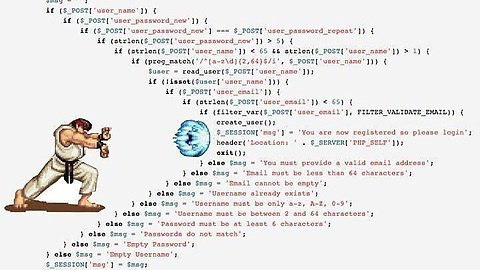
\includegraphics[height=0.7\paperheight]{ryu.jpg}
  \end{center}
\end{frame}


\begin{frame}{Syntactic sugar (\texttt{do}-notation):}
  \texttt{
    \ \ do result <- action \\
    \ \ \ \ \ \ actions  ... \\
  } \ \\ \pause
  is transformed to: \\ \pause
  \texttt{
    \ \ pass action (λ result -> do actions ...) \\
  } \ \\  \pause
  \ \\
  Note: In Haskell, \texttt{pass} is written down as
  \texttt{>>=} and pronounced ``bind''.
\end{frame}

\begin{frame}{Relation between \texttt{pass} and \texttt{<|}}
  \pause
  \texttt{pass$_m$ :: $m$ a -> (a -> $m$ b)} \\ \pause
  \texttt{<|$_m$ ::\ (b -> $m$ c) -> (a -> $m$ b) -> (a -> $m$ c)} \\ \pause
  \texttt{pass value function = (function <| id) value} \\ \pause
  \texttt{(f <| g) x = pass (g x) f} \\ \pause
  \texttt{return$_m$ :: (a -> $m$ a)} \\ \pause
  \texttt{return$_m$ = id$_m$}
\end{frame}

\end{document}
